\section{Problemas de satisfacción de restricciones}

\subsection{Definición}

\begin{definition}
Un problema de satisfacción de restricciones está definido por:
 \begin{itemize}
  \item Un conjunto de variables $\set{V} = \{X_1,X_2,...,X_n\}$
  \item Un conjunto de restricciones $\set{C} = \{C_1,C_2,...,C_m\}$
  \item Cada variable tiene un dominio asociado $\mathbb{D}_v$ con $\mathbb{D}_v \neq \emptyset$
 \end{itemize}
\end{definition}

Para este tipo de problemas 
\begin{itemize}
\item Un estado es una asignación a unas o todas las variables $\set{S} = \{X_i = v_i, X_j=v_j,...\}$
\item Una \emph{asignación consistente} es una asignación que no viola ninguna restricción.
\item Una \emph{asignación completa} es una asignación que menciona a todas las variables.
\item Una solución es una asignación completa y consistente.
\end{itemize}

Entonces el sistema de transiciones en el espacio de estados $\Sigma=(\set{S},\set{A},\gamma)$, queda definido con los elementos siguientes:
\begin{itemize}
 \item $\set{S}= \{s_1,s_2,...\}$ el conjunto de todas las posibles asignaciones (parciales y completas) a las variables del problema.
 \item $\set{A}= \{a_1,a_2,...\}$ el conjunto de las acciones que asignan a alguna variable $X_i$ un valor $v$ del dominio $\mathbb{D}_{X_i}$.
 \item $\gamma: S \times A \rightarrow S$ la función que aplica la acción $a_i$ en el estado $s_j$, si al realizar la asignación $a_i$, $s_j$ no queda en un estado inconsistente.  Para todos los demás casos, devuelve $\emptyset$ y se dice que la acción no es aplicable.
\end{itemize}

De este modo, el problema de planeación $\mathcal{P} = (\Sigma, s_i,g)$ usa:
  
\begin{itemize}
  \item $s_i = \{\}$ la asignación vacía.
  \item $g(s)$ la función que verifica si la asignación es completa.
\end{itemize}




\subsection{Recorrido en el espacio de búsqueda}

Para mostrar cómo se realiza una búsqueda en este espacio se utilizará el problema del \textit{Sudoku}.  Utilicemos como ejemplo el tablero mostrado en la \fref{fig:sudoku_vacio}.

\begin{figure}
 \centering
 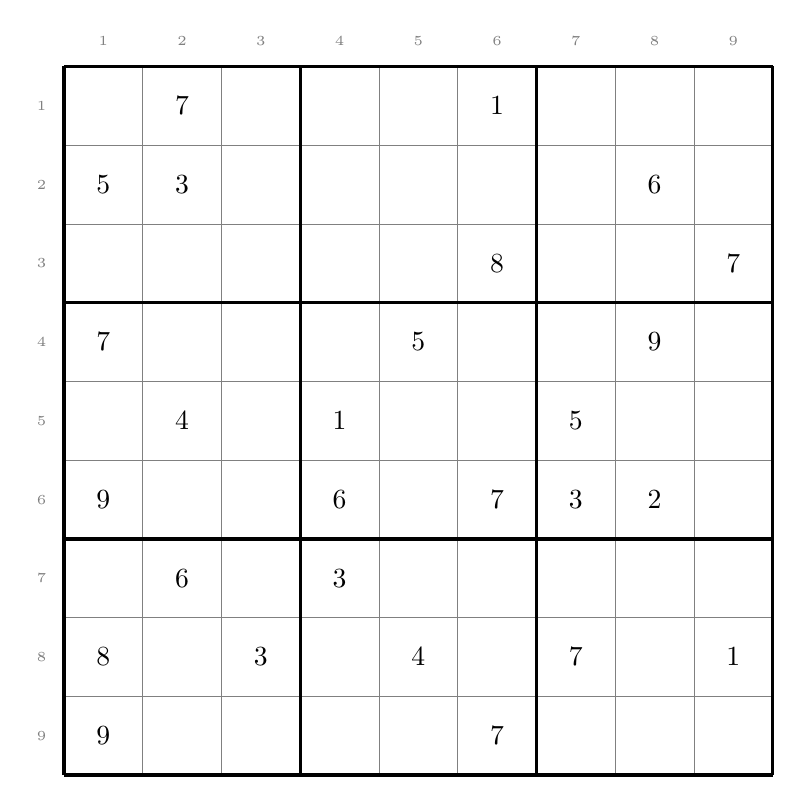
\begin{tikzpicture}
  \draw[step=1cm,gray,very thin] (0,0) grid (9,9);
  \draw[step=3cm,black,very thick] (0,0) grid (9,9);
  
  \node at (0.5cm,0.5cm) {9};
  \node at (5.5cm,0.5cm) {7};
  
  \node at (0.5cm,1.5cm) {8};
  \node at (2.5cm,1.5cm) {3};
  \node at (4.5cm,1.5cm) {4};
  \node at (6.5cm,1.5cm) {7};
  \node at (8.5cm,1.5cm) {1};
  
  \node at (1.5cm,2.5cm) {6};
  \node at (3.5cm,2.5cm) {3};
  
  \node at (0.5cm,3.5cm) {9};
  \node at (3.5cm,3.5cm) {6};
  \node at (5.5cm,3.5cm) {7};
  \node at (6.5cm,3.5cm) {3};
  \node at (7.5cm,3.5cm) {2};
  
  \node at (1.5cm,4.5cm) {4};
  \node at (3.5cm,4.5cm) {1};
  \node at (6.5cm,4.5cm) {5};

  \node at (0.5cm,5.5cm) {7};
  \node at (4.5cm,5.5cm) {5};
  \node at (7.5cm,5.5cm) {9};
  
  \node at (5.5cm,6.5cm) {8};
  \node at (8.5cm,6.5cm) {7};
  
  \node at (0.5cm,7.5cm) {5};
  \node at (1.5cm,7.5cm) {3};
  \node at (7.5cm,7.5cm) {6};
  
  \node at (1.5cm,8.5cm) {7};
  \node at (5.5cm,8.5cm) {1};
  
  \foreach \j in {1,...,9} { \node [anchor=north,gray] at (\j-0.5,9.5) {\tiny \j}; }
  \foreach \y [evaluate=\y as \i using int(10-\y)] in {1,...,9} { \node [anchor=east,gray] at (-0.1,\y-0.5) {\tiny \i}; }
 \end{tikzpicture}
 \caption{Tablero de Sudoku al iniciar un juego.}\label{fig:sudoku_vacio}
\end{figure}

En este escenario, las variables son las casillas vacías del Sudoku.  Sea $\set{X}$ el conjunto de todas las casillas.  Identifiquemos a cada casilla con el símbolo $X_{ij}$, con $i$ y $j$ en $\{1,2,...,9\}$, según su posición en el tablero.  Los valores posibles para cada casilla están en $\mathbb{D}_v = \{1,2,...,9\}$.

Dado que el juego del Sudoku comienza con valores en algunas casillas, el estado inicial ya tiene valores asociados a algunas de las $X_{ij}$.  Para el tablero del ejemplo se tendría la asignación inicial $F$:

\begin{align*}
 F = \{
 X_{12} =& 7,   &   X_{16} =& 1, \\
 X_{21} =& 5,   &   X_{22} =& 3,   &   X_{28} =& 6, \\
 ... \\
 X_{81} =& 8,   &   X_{83} =& 3,   &   X_{85} =& 4,   &   X_{87} =& 7,   &   X_{89} =& 1, \\
 X_{91} =& 9,   &   X_{96} =& 7\} \\
\end{align*}

Sin embargo, dado que los valores de estas casillas no pueden ser cambiados, este conjunto de casillas no pertenece al conjunto de variables.  Más bien se tiene:
\begin{align*}
 \set{V} = \set{X} - \set{F}
\end{align*}

Estimemos la complejidad inicial de este problema, calculando el número de estados posibles con asignaciones completas:
\begin{enumerate}
 \item Hay $|V|$ casillas vacías, cada una de las cuales puede albergar $9$ valores distintos.
 \item Esto da un total de $9^{|V|}$ asignaciones posibles.
\end{enumerate}
En el ejemplo anterior, son $9^{54} \approx 3.5\times10^{51}$.  Compárese con la capacidad de un disco duro de un terabyte, donde $1\unit{T} \approx 10^{12} \unit{bytes}$.  No intentemos siquiera agregar las asignaciones incompletas.  Claramente no es posible resolver este problema sin hacer uso de las restricciones, para evitar recorrer este espacio de estados.

\subsubsection{Propagación de restricciones}

Por la forma en que se planteó el problema en la sección anterior, se comienza la búsqueda de un solución, con la asignación vacía $s_i = \{\}$.  ¿Cuáles son las acciones aplicables en este momento?  Para comenzar: las acciones posibles son aquellas que asignan un valor a alguna de las casillas vacías.  Obsérvese que se estableció como precondición para su aplicabilidad, que el valor asignado no viole ninguna de las restricciones del problema.  En el caso del Sudoku, éstas son:
\begin{enumerate}
 \item Que no haya otra casilla en el mismo renglón, con el mismo valor.
 \item Que no haya otra casilla en la misma columna, con el mismo valor.
 \item Que no haya otra casilla en el mismo cuadrante, con el mismo valor.
\end{enumerate}

Consideremos ahora al conjunto $\mathbb{D}_v$ de valores posibles para cada variable.
Estas tres condiciones implican que, cada vez que se asigne un valor $v$, a una casilla $X_{ij}$, los valores que permiten una asignación consistente se reducen para las casillas siguientes:
\begin{enumerate}
 \item Todas las casillas en el renglón $i$, ya no pueden tener a $v$ como valor.
 \item Todas las casillas en la columna $j$, ya no pueden tener a $v$ como valor.
 \item Todas las casillas en el cuadrante $i$, ya no pueden tener a $v$ como valor.
\end{enumerate}

Antes de elegir la acción a aplicar, es necesario \emph{propagar} el efecto de estas restricciones, para determinar cuáles son las acciones aplicables en un estado dado.  Depués de hacer esto, quedarán grupos de acciones aplicables: un grupo por cada variable que aún no ha sido asignada, con tantas acciones asociadas, como valores sea posible asignarle.  Visualicemos esto como en la \fref{fig:sucesores_restricciones}.

\begin{figure}
 \centering
 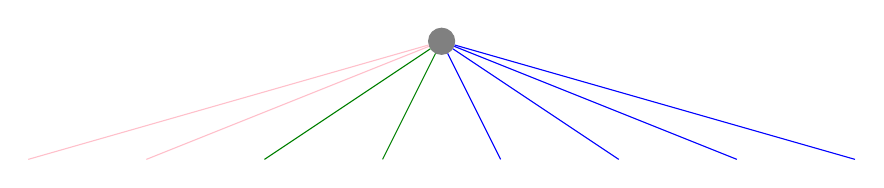
\begin{tikzpicture}
  \node [circle, fill=Gray, draw=Gray] {}
    child [circle, fill=Pink, draw=Pink] {}
    child [circle, fill=Pink, draw=Pink] {}
    child [circle, fill=Green, draw=Green] {}
    child [circle, fill=Green, draw=Green] {}
    child [circle, fill=Blue, draw=Blue] {}
    child [circle, fill=Blue, draw=Blue] {}
    child [circle, fill=Blue, draw=Blue] {}
    child [circle, fill=Blue, draw=Blue] {}
  ;
 \end{tikzpicture}
 \caption{Grupos de acciones aplicables y sus sucesores para un problema de satisfacción de restricciones.}\label{fig:sucesores_restricciones}
\end{figure}

Todas las variables que no han sido asignadas deberán recibir alguna asignación en algún momento.  Sin embargo, podemos seleccionar cual asignaremos primero y esto acelerará la búsqueda drásticamente.  También podemos elegir qué valor probaremos primero, de entre los que aún se le puede asignar.  Hay tres reglas que sugieren cómo realizar estas elecciones:
